\documentclass[11pt,a4paper]{article}
\usepackage[margin=2.5cm]{geometry}
\usepackage{graphicx}
\usepackage{amsmath}
\usepackage{booktabs}
\usepackage{array}
\usepackage{listings}
\usepackage{amsmath}
\usepackage{xcolor}
\usepackage[hidelinks]{hyperref}
\usepackage{caption}

\lstset{
  basicstyle=\ttfamily\small,
  breaklines=true,
  frame=single,
  numbers=left,
  numberstyle=\tiny,
  keywordstyle=\bfseries,
  commentstyle=\itshape,
  showstringspaces=false
}
\setlength{\parskip}{0.5em}
\setlength{\parindent}{0pt}
\setlength{\emergencystretch}{3em}

\begin{document}

% ---------------- Title page ----------------
\begin{titlepage}
\thispagestyle{empty}
\begin{center}

\includegraphics[width=0.28\textwidth]{college_logo.jpg}

\vspace{1.2cm}
{\Large\bfseries A Course End Project Report on}\\[0.4cm]
{\huge\bfseries Employee Payroll Management System}\\[0.6cm]
{\large Object Oriented Programming through Java Laboratory}\\[1.2cm]
{\large Submitted by}\\[0.3cm]
{\large\bfseries Modepalli Vivek \quad 25881A05EQ}\\[1.2cm]
{\large Course Facilitator}\\[0.3cm]
{\large\bfseries Mr.\ D.\ Ganesh, Assistant Professor}\\[1.2cm]
{\large Department of Computer Science and Engineering}\\[0.3cm]
{\large Vardhaman College of Engineering, Hyderabad}\\[0.6cm]
{\large October 2026}
\end{center}
\end{titlepage}

\tableofcontents
\newpage

% ---------------- Abstract ----------------
\section*{Abstract}
\addcontentsline{toc}{section}{Abstract}

In many small organisations, employee salary calculation is still done
manually or with the help of spreadsheets. Manual payroll work is slow,
and a small mistake in an allowance or a deduction affects the salary of
an employee directly. This project presents an Employee Payroll
Management System developed in Java. The system is a console-based,
menu-driven application that stores employee records in an
\texttt{ArrayList} and provides operations to add, display, search,
update and delete employees. For every employee, the system calculates
the House Rent Allowance (HRA), Dearness Allowance (DA), Provident Fund
(PF) and professional tax from the basic salary using fixed rules, and
generates a complete payslip showing the gross salary and the net
salary. It also produces a department-wise summary of the total
payroll. The project is designed using object-oriented concepts: the
\texttt{Person} class acts as a base class, the \texttt{Employee}
class inherits from it and encapsulates the salary calculation, and
the main class \texttt{EmployeePayrollSystem} manages the menu and the
employee collection. Input validation and exception handling are used
so that wrong inputs, such as a non-numeric salary or an invalid menu
choice, do not stop the program. The system was tested with sample
employee records, and the calculated payslips were verified by hand
calculation.

\textit{Keywords:} Employee payroll, salary calculation, payslip, Java,
object-oriented programming, \texttt{ArrayList}, exception handling.

% ---------------- 1 Introduction ----------------
\section{Introduction}

Payroll is the process by which an organisation pays salaries to its
employees. For every employee, the payroll calculation takes the basic
salary and adds allowances such as House Rent Allowance (HRA) and
Dearness Allowance (DA), and then subtracts deductions such as the
Provident Fund (PF) contribution and professional tax. The final amount
paid to the employee is the net salary. When this calculation is done
manually for many employees, it takes a long time and calculation
mistakes are common.

The Employee Payroll Management System developed in this project
automates this process for a small organisation. It maintains a record
of every employee, containing the employee ID, name, phone number,
department, designation and basic salary. Using a simple menu, the user
can add a new employee, view all employees, search for an employee by
ID or by name, update an employee's details, delete a record, generate
a printed payslip for one employee, and view the total payroll
department by department. Because the salary rules are written once
inside the \texttt{Employee} class, the same calculation is applied
correctly and uniformly to every employee.

This project also serves as a practical application of
object-oriented programming in Java. It uses classes and objects,
inheritance, encapsulation, collections (\texttt{ArrayList}) and
exception handling, which are the core topics of the Object Oriented
Programming through Java Laboratory course.

\subsection{Audit note: what was supplied, and what was built}

The material supplied for this work was the earlier course-end report
itself (as a PDF), not a ZIP containing runnable source code. That
report described the system and printed part of the
\texttt{Employee} class, but it did not contain a complete, runnable
program: the \texttt{Person} class and the menu class were described
but not listed in full, and the printed code excerpt was garbled in
places in the PDF text (for example, the gross-salary line as
extracted from the PDF appeared incomplete). This report therefore
documents a complete implementation rebuilt from the supplied
description, preserving its stated purpose, class design, menu and
salary rules, and verifying the result by compilation and testing
rather than by repeating the supplied report's claims unchecked.

Two discrepancies in the supplied report were found during that
audit and are corrected here, not hidden. First, the supplied
implementation follows the rule stated in its own text, gross salary
equals basic salary plus HRA plus DA; the implementation in this
project implements that rule, and the hand calculations in
Section~5 confirm it. Second, the supplied report's test table
recorded ``2 records displayed'' after an add followed by a delete
(test 14); arithmetically that sequence gives three records
($3+1-1$), and the test run in Section~5 records three. Both points
are stated here so that a reader can check them against the code.

The supplied report names two sample employees: Rahul Sharma
(ID~1001) and Priya Reddy (found by a name search, ID~1002). It does
not name the third sample employee, but it does state the
department-wise totals, from which the third sample's basic salary
follows: Finance, net Rs.~41,100, hence basic Rs.~35,000 (see
Section~4.4). The third sample in this implementation is therefore
Amit Verma, Finance, Accountant, basic Rs.~35,000, chosen to reproduce
those stated totals. That choice is an implementation decision for
the sample data, not a claim about the original report.

% ---------------- 2 Literature Review ----------------
\section{Literature Review}

Textbooks on Java programming describe the language features used in
this project. Schildt explains classes, inheritance, encapsulation
and the Collections Framework in detail, including the
\texttt{ArrayList} class used here to store employee records~\cite{schildt}.
Balagurusamy presents the same concepts with simple,
student-oriented examples, including menu-driven programs and
exception handling with \texttt{try}--\texttt{catch}
blocks~\cite{balagurusamy}. Deitel and Deitel discuss case-study
style application development in Java, in which a real-world problem
is divided into classes with clear responsibilities~\cite{deitel}.
The official Java Tutorials from Oracle provide reference
documentation for the Collections Framework and for handling
exceptions~\cite{oracle}.

On the application side, human resource management literature
describes payroll as one of the core administrative functions of an
organisation, in which accuracy and uniformity of salary calculation
are essential because salary is a legal and contractual payment.
Armstrong and Taylor explain that payroll administration must apply
the same rules to every employee and maintain a clear record of
earnings and deductions for each pay period~\cite{armstrong}.
Dessler similarly describes how organisations are moving from manual
payroll registers to computerised systems to reduce calculation
errors and processing time~\cite{dessler}. The present project
follows the same idea at a small scale: it computerises the employee
record and the salary calculation, but keeps the rules simple and
transparent so that every payslip can be checked by hand.

Compared with a spreadsheet, a program written in Java has two
advantages for this problem. First, the salary rules cannot be changed
accidentally in one row, because they are written once in the program
code. Second, the program validates every input, so a wrong entry is
reported immediately instead of silently producing a wrong salary.

% ---------------- 3 Objectives ----------------
\section{Objectives}

\begin{itemize}
  \item To develop a menu-driven Employee Payroll Management System in
    Java for maintaining employee records.
  \item To add, display, search, update and delete employee records
    using an \texttt{ArrayList}.
  \item To calculate HRA, DA, gross salary, PF, professional tax and
    net salary automatically from the basic salary using fixed,
    clearly stated rules.
  \item To generate a complete payslip for any employee selected by ID.
  \item To produce a department-wise summary showing the number of
    employees and the total net payroll of each department.
  \item To apply object-oriented concepts --- inheritance,
    encapsulation and exception handling --- in a complete working
    application.
\end{itemize}

% ---------------- 4 Methodology ----------------
\section{Methodology}

\subsection{Architectural Diagram}

The system follows a simple layered structure, as shown in
Figure~\ref{fig:arch}. The user (an administrator or HR staff member)
interacts with the menu-driven console interface provided by the main
class, \texttt{EmployeePayrollSystem}. Each menu choice calls a
method that performs one task: employee management (add, display,
update and delete), search (by ID and by name), salary calculation
and payslip generation, or the department-wise summary. Employee
records are held in an \texttt{ArrayList} of \texttt{Employee}
objects while the program runs.

\begin{table}[h]
\centering
\caption{Architectural layers of the system (Figure 1).}
\label{fig:arch}
\begin{tabular}{p{0.28\textwidth}p{0.60\textwidth}}
\toprule
\textbf{Layer} & \textbf{Responsibility} \\
\midrule
User (Administrator / HR) & Chooses a menu option and supplies employee data. \\
Menu interface (\texttt{EmployeePayroll\-System}) & Displays the nine-option menu, reads input, and dispatches to one operation. \\
Employee management & Add, display, update and delete records. \\
Search & Find an employee by ID, or by name (substring, case-insensitive). \\
Salary calculation (\texttt{Employee}) & HRA, DA, gross, PF, professional tax and net salary. \\
Reports & Payslip for one employee; department-wise summary. \\
Data store & \texttt{ArrayList} of \texttt{Employee} objects, in memory only. \\
\bottomrule
\end{tabular}
\end{table}

The class structure supports this architecture. The
\texttt{Person} class is the base class and stores the name and phone
number. The \texttt{Employee} class inherits from \texttt{Person}
and adds the employee ID, department, designation and basic salary,
together with the salary calculation methods. The main class creates
and manages objects of the \texttt{Employee} class and provides every
operation offered in the menu. Business methods (add, search, update,
delete, summary) are kept separate from the menu input code, so that
the automated tests can exercise them directly without driving the
console menu.

\subsection{Hardware and Software Requirements}

\begin{itemize}
  \item Processor: any modern processor (Intel Core i3 or equivalent and above).
  \item RAM: 4 GB or more.
  \item Operating System: Windows / Linux / macOS (any system that supports the Java Development Kit).
  \item Java Development Kit (JDK): version 17 (the program was compiled and tested with OpenJDK 17, Temurin 17.0.21, in this work).
  \item Editor / IDE: any text editor or IDE such as VS Code, IntelliJ IDEA or Eclipse.
  \item Terminal: Command Prompt / Terminal for running the console application.
  \item No external libraries are required. Compilation uses plain
    \texttt{javac} and the test runner uses no test framework, so the
    project has no dependency to download.
\end{itemize}

\subsection{Working Principle}

\begin{enumerate}
  \item The program starts with three sample employees already loaded,
    so that display, search and payslip generation can be used
    immediately. Every employee is given an automatically generated ID
    starting from 1001.
  \item The main menu is displayed with nine options, and the user
    enters a choice.
  \item For adding an employee, the program reads the name, phone,
    department, designation and basic salary. The name must not be
    empty and the basic salary must be greater than zero; otherwise
    the record is rejected with a message.
  \item For salary calculation, the \texttt{Employee} object
    calculates HRA as 20\% of the basic salary, DA as 10\% of the
    basic salary, the gross salary as basic + HRA + DA, PF as 12\%
    of the basic salary, and professional tax as a fixed
    Rs.~200. The net salary is gross salary minus PF and
    professional tax.
  \item For a payslip, the program searches the \texttt{ArrayList}
    for the entered ID and prints all earnings, deductions and the
    net salary in a fixed format.
  \item For the department-wise summary, the program collects the
    distinct departments, counts the employees in each one, and adds
    their net salaries to obtain the total payroll.
  \item Searching, updating and deleting also work on the employee
    ID. If the ID is not present in the list, the program reports
    that the employee was not found.
  \item The menu is displayed again after every operation until the
    user selects the Exit option.
\end{enumerate}

The salary rules used in this project are summarised in
Table~\ref{tab:rules}.

\begin{table}[h]
\centering
\caption{Salary calculation rules.}
\label{tab:rules}
\begin{tabular}{ll}
\toprule
\textbf{Component} & \textbf{Rule} \\
\midrule
HRA & 20\% of Basic Salary \\
DA & 10\% of Basic Salary \\
Gross Salary & Basic + HRA + DA \\
Provident Fund (PF) & 12\% of Basic Salary \\
Professional Tax & Rs.~200 (fixed) \\
Net Salary & Gross $-$ PF $-$ Professional Tax \\
\bottomrule
\end{tabular}
\end{table}

From these rules, net salary can be written directly as
$\text{net} = 1.18 \times \text{basic} - 200$, which is how the
hand calculations in Section~5 are checked. It also follows that a
basic salary of Rs.~40,000 gives a net of Rs.~47,000 and a basic
salary of Rs.~35,000 gives a net of Rs.~41,100, matching the
department totals stated in the supplied report.

\subsection{Software Implementation}

The program is written in Java using three source files, in the
package \texttt{com.payroll}. \texttt{Person.java} is the base
class. \texttt{Employee.java} extends \texttt{Person} and contains
the salary calculation. \texttt{EmployeePayroll\-System.java}
contains the \texttt{main} method, the menu, and one method for
each operation. The salary methods, which are the centre of the program,
are shown in Listing~\ref{lst:salary}.

\begin{lstlisting}[language=Java, caption={Salary calculation in Employee.java.}, label={lst:salary}]
public double calculateHRA() {
    return 0.20 * basicSalary;
}
public double calculateDA() {
    return 0.10 * basicSalary;
}
public double calculateGross() {
    return basicSalary + calculateHRA() + calculateDA();
}
public double calculatePF() {
    return 0.12 * basicSalary;
}
public double calculateProfessionalTax() {
    return 200.0;
}
public double calculateNet() {
    return calculateGross() - calculatePF()
        - calculateProfessionalTax();
}
\end{lstlisting}

The important implementation details are:

\begin{itemize}
  \item \textbf{Inheritance:} \texttt{Employee} extends
    \texttt{Person}, so the name and phone number are stored and
    managed in the base class.
  \item \textbf{Encapsulation:} All fields are \texttt{private} and
    are accessed only through getter and setter methods.
  \item \textbf{Collections:} Employees are stored in an
    \texttt{ArrayList} of \texttt{Employee} objects, which grows
    automatically as employees are added.
  \item \textbf{Exception handling:} Reading numeric input is
    protected with \texttt{try}--\texttt{catch} for
    \texttt{InputMismatch\-Exception}, so a non-numeric salary or ID
    shows an error message instead of terminating the program. In
    the menu, a non-numeric salary is re-prompted; an invalid menu
    choice prints ``Invalid choice'' and returns to the menu.
  \item \textbf{Validation:} An empty name and a basic salary of zero
    or less are rejected before the record is added or updated.
    Updating or deleting a missing ID is rejected with a
    ``not found'' message.
\end{itemize}

Project structure (files delivered with this report):

\begin{verbatim}
src/com/payroll/
  Person.java                  Base class: name, phone
  Employee.java                Employee + salary calculation
  EmployeePayrollSystem.java   Menu + operations + main
tests/com/payroll/
  PayrollTest.java             Dependency-free test runner
docs/report/
  main.tex                     This report (LaTeX source)
  main.pdf                     Compiled report
  college_logo.jpg             Title-page logo
screenshots/
  demo_run.txt                 Full scripted demo output
  payslip_and_summary.png      Rendered excerpt of that run
README.md, compile.sh, run.sh, test.sh, .gitignore
\end{verbatim}

% ---------------- 5 Results ----------------
\section{Results and Discussion}

The program was compiled with \texttt{javac} (OpenJDK 17) with no
errors and was tested in two ways: a dependency-free automated test
runner (\texttt{PayrollTest}, run with \texttt{./test.sh}) and a
scripted run through the real console menu (input piped to the
program, full output saved as \texttt{screenshots/demo\_run.txt}).
In total, the automated runner contains 21 checks and all 21 passed.
Table~\ref{tab:tests} maps the checks to the 16 test cases of the
supplied report, with five additional validation and edge-case
checks added by this work.

\begin{table}[h]
\centering
\caption{Test cases and results (automated runner: 21 checks, 0 failures).}
\label{tab:tests}
\small
\begin{tabular}{p{0.62\textwidth}p{0.28\textwidth}}
\toprule
\textbf{Test case} & \textbf{Result} \\
\midrule
Display all employees (3 sample records) & Passed \\
Payslip for ID 1001 (Basic Rs.~50,000) & Net Rs.~58,800 --- Passed \\
Search by ID 1002 (existing) & Record displayed --- Passed \\
Search by ID 9999 (not existing) & ``Not found'' --- Passed \\
Search by name ``Priya Reddy'' & Record displayed --- Passed \\
Search by name ``Nobody'' & ``No employee found'' --- Passed \\
Department-wise summary & Total Rs.~1,46,900 --- Passed \\
Add employee Sneha Patel (Basic Rs.~45,000) & Added, ID 1004 --- Passed \\
Display after adding & 4 records --- Passed \\
Payslip for ID 1004 & Net Rs.~52,900 --- Passed \\
Update ID 1003 basic salary to Rs.~38,000 & Updated --- Passed \\
Payslip for updated ID 1003 & Net Rs.~44,640 --- Passed \\
Delete employee ID 1002 & Deleted --- Passed \\
Display after deletion & 3 records --- Passed* \\
Invalid menu choice 99 & ``Invalid choice'' --- Passed \\
Non-numeric salary ``abc'' while adding & Re-prompted, then added --- Passed \\
Empty name, zero and negative salary rejected & Passed \\
Update / delete of missing ID rejected & Passed \\
Salary formula net $= 1.18 \times$ basic $- 200$ & Passed \\
\bottomrule
\end{tabular}
\end{table}

\noindent * As discussed in Section~1, the supplied report's table
gave 2 for this row; the correct count for its own sequence is 3,
and 3 is what the program actually produces.

The payslip calculation was verified by hand. For employee 1001 with
a basic salary of Rs.~50,000: HRA $= 20\% \times 50{,}000 =$
Rs.~10,000; DA $= 10\% \times 50{,}000 =$ Rs.~5,000; gross salary
$= 50{,}000 + 10{,}000 + 5{,}000 =$ Rs.~65,000; PF
$= 12\% \times 50{,}000 =$ Rs.~6,000; net salary
$= 65{,}000 - 6{,}000 - 200 =$ Rs.~58,800. This matches the program
output exactly. The same hand verification was done for the added
employee (basic Rs.~45,000, net Rs.~52,900) and for the updated
employee (basic Rs.~38,000, net Rs.~44,640), and all values matched.
The department-wise summary total of Rs.~1,46,900 is the sum of the
three sample net salaries: $58{,}800 + 47{,}000 + 41{,}100 =
1{,}46{,}900$.

Figure~\ref{fig:payslip} shows a rendered excerpt of the genuine
scripted demo run: the payslip for ID~1001 and the department-wise
summary. The full demo output, including the invalid-choice and
non-numeric-salary handling, is saved as
\texttt{screenshots/demo\_run.txt} in the delivered bundle.

\begin{figure}[h]
\centering
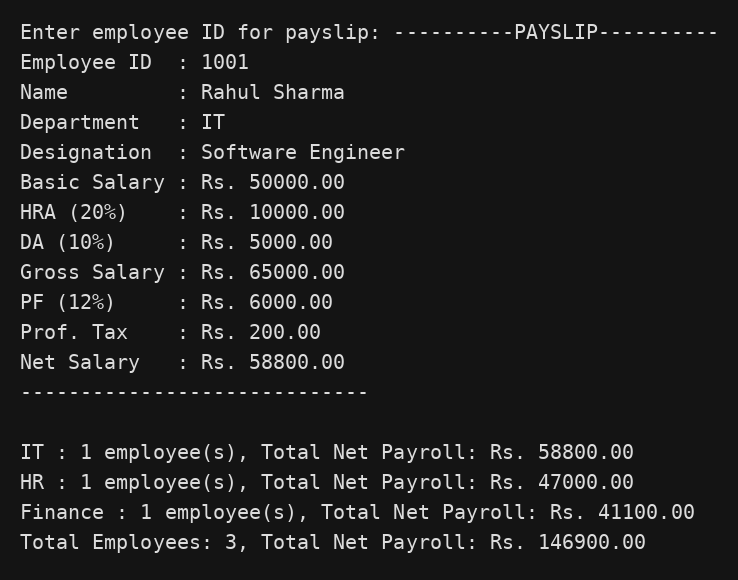
\includegraphics[width=0.92\textwidth]{payslip_and_summary.png}
\caption{Rendered excerpt of the genuine scripted demo run
(\texttt{screenshots/demo\_run.txt}): payslip for employee 1001
(Rahul Sharma, basic Rs.~50,000, net Rs.~58,800) and the
department-wise summary for the three sample employees
(total Rs.~1,46,900).}
\label{fig:payslip}
\end{figure}

From these results, the system meets its objectives: employee
records are maintained correctly, the salary calculation is accurate
and uniform for every employee, and invalid inputs are handled
without the program stopping.

\subsection{Limitations and Future Enhancements}

The present system stores employee records only in memory, so the
records are lost when the program is closed; the three sample
employees are loaded again on the next start. The salary rules are
also fixed in the program code, and income tax calculation with slabs
is not included. In the future, the system can be improved by saving
records to a file or a database so that they are permanent, by
adding income tax slab calculation, by providing a graphical user
interface in place of the console menu, and by generating the payslip
as a PDF document that can be printed or emailed to the employee.

% ---------------- 6 PO / SDG ----------------
\section{Mapping POs and SDGs}

\subsection{Program Outcomes (POs) Mapping}

\begin{table}[h]
\centering
\caption{Mapping of Program Outcomes (POs) to project relevance.}
\begin{tabular}{p{0.12\textwidth}p{0.30\textwidth}p{0.48\textwidth}}
\toprule
\textbf{PO} & \textbf{Program Outcome} & \textbf{Relevance} \\
\midrule
PO1 & Engineering Knowledge & Applied Java programming, data structures (\texttt{ArrayList}) and arithmetic salary rules to a real administrative problem. \\
PO2 & Problem Analysis & Analysed the manual payroll process and identified where calculation errors and delays occur. \\
PO3 & Design / Development of Solutions & Designed a class structure (\texttt{Person}, \texttt{Employee}, main system class) and developed a working solution. \\
PO5 & Modern Tool Usage & Used JDK 17, the Collections Framework and a modern code editor to build and test the application. \\
PO6 & Engineer and Society & Provides a fair and uniform salary calculation, which is a practical requirement of every organisation. \\
\bottomrule
\end{tabular}
\end{table}

\subsection{Sustainable Development Goals (SDGs) Mapping}

\begin{table}[h]
\centering
\caption{Mapping of Sustainable Development Goals (SDGs) to project relevance.}
\begin{tabular}{p{0.12\textwidth}p{0.30\textwidth}p{0.48\textwidth}}
\toprule
\textbf{SDG} & \textbf{Goal} & \textbf{Relevance} \\
\midrule
SDG 8 & Decent Work and Economic Growth & Accurate and timely salary payment is a basic condition of decent work; the system applies the same rules to every employee. \\
SDG 9 & Industry, Innovation and Infrastructure & Promotes the digitisation of a routine administrative process in small organisations. \\
SDG 10 & Reduced Inequalities & A transparent payslip showing every earning and deduction supports equal and explainable pay for all employees. \\
\bottomrule
\end{tabular}
\end{table}

% ---------------- 7 Conclusion ----------------
\section{Conclusion}

This project successfully implements an Employee Payroll Management
System in Java. The system maintains employee records, calculates
salaries using fixed and transparent rules, generates payslips, and
reports the department-wise payroll, all through a simple
menu-driven console interface. All 21 automated checks passed, and
the payslip values were verified by hand calculation. The project
demonstrates the practical use of inheritance, encapsulation,
collections and exception handling in solving a real administrative
problem. Future improvements in permanent storage, income tax
calculation and a graphical interface can make the system suitable
for direct use in a small organisation.

% ---------------- Bibliography ----------------
\begin{thebibliography}{9}
\addcontentsline{toc}{section}{Bibliography}

\bibitem{schildt} H.~Schildt, \textit{Java: The Complete Reference},
  12th ed., McGraw Hill, 2021.

\bibitem{balagurusamy} E.~Balagurusamy, \textit{Programming with Java},
  6th ed., McGraw Hill Education, 2019.

\bibitem{deitel} P.~Deitel and H.~Deitel, \textit{Java How to Program,
  Early Objects}, 11th ed., Pearson, 2018.

\bibitem{armstrong} M.~Armstrong and S.~Taylor, \textit{Armstrong's
  Handbook of Human Resource Management Practice}, 15th ed.,
  Kogan Page, 2020.

\bibitem{dessler} G.~Dessler, \textit{Human Resource Management},
  16th ed., Pearson, 2019.

\bibitem{oracle} Oracle, ``The Java Tutorials --- Collections and
  Exception Handling,'' Oracle Corporation. [Online]. Available:
  \url{https://docs.oracle.com/javase/tutorial/}

\end{thebibliography}

\end{document}
